\subsection{Menubar}
In eCAD we have menubar. In menubar it contains different menu items and sub menuitems. Each menuitem has its own specific requirement and advantage. Each menu item is described as below:
\begin{figure}[h!]
\centering
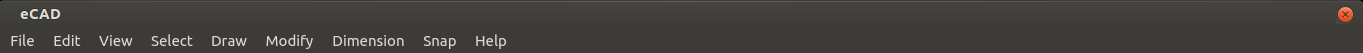
\includegraphics[width=0.9\textwidth]{images/menubar.png}
\caption{Menubar}
\end{figure}
\begin{enumerate}
\item \textbf{File Menu}: It contains following submenus.
\begin{itemize}
\item New: On clicking this menuitem we can create a new document. The shortcut key to is Ctrl+N
\item Open: This is used to open a file which was already saved, so that we can edit that file as per user requiremenet. The shortcut key is Ctrl+O
\item Save: On clicking this we get our file save in xml format. The shorcut to this is Ctrl+S
\item Save As: When one wants to save the file with different name. He/She can do so with Save As functionality. The shorcut to it is Ctrl+Shift+S
\item Import: Using this one can import the file from outside souce. One can import jpg and png images in eCAD
\item Export: Also once file is made need to be exported. In eCAD one can export the file in the pdf, jpg and png format.
\item Close: On clicking this the current document gets close.
\item Print preview: Before printing user may want to view the file to print. This can be done by clicking on it or by pressing Ctrl+Shift+P 
\item Print: To print the file click on it or press Ctrl+P.
\item Quit: To quit or close the software click on it or press Ctrl+Q
\end{itemize}
\item \textbf{Edit Menu}: It contains following submenus
\begin{itemize}
\item Cut: To cut the item click on this or press Ctrl+X
\item Copy: To copy the item click on this or press Ctrl+C
\item Paste: To paste the item click on this or press Ctrl+V
\item Undo: To Undo click on it or press Ctrl+Z
\item Redo: To Redo click on it or press Ctrl+Shift+Z
\end{itemize}
\item \textbf{View menu}: It contains following submenus
\begin{itemize}
\item Grid: On clicking this Grid appears and disappears
\item Zoom In: On clicking this the view gets zoom in
\item Zoom out: On clicking this the view gets zoom out
\item Panning: One can move the screen using this feature
\item Status Bar: This shows the current screen position and also what to do next after clicking on entities. 
\item Tool Bar: It futher have submenus for toolbar, scripting widgets and console mode.
\end{itemize}
\item \textbf{Select}: It contains following submenus
\begin{itemize}
\item Select all: This will select all the entities
\item Deselect all: This will deselect all entites 
\item Select Window: This will select full window
\item Select entity: This will allow to select one entity
\item Deselect window: This will deselect window 
\item Invert Selection: This will invert the selection.
\end{itemize}
\item \textbf{Draw}: It contains following submenus
\begin{itemize}
\item Points: It is used to add points.
\item Line: It is used to draw Line
\item Circle: It is used to draw Circle
\item Ellipse: It is used to add the ellipse
\item Arc: It is used to add the arc
\item Text: It is used to add the text
\item Image: It is used to add the image
\end{itemize}
\item \textbf{Modify} : It contains following submenus.
\begin{itemize}
\item Delete selected: It will delete the selected items.
\item Delete entity: It will delete the single entity. 
\end{itemize}
\item \textbf{Dimension}: It contains following submenus
\begin{itemize}
\item Horizontal: It will add the horizontal dimension.
\item Vertical: It will add the vertical dimension. 
\end{itemize}
\item \textbf{Snap}: It contains following submenus
\begin{itemize}
\item Free: It will be free snap.
\item Grid: It will be for snap to grid. 
\item Center: It will be for snap to center
\item Middle Points: It will be for snap to mid points
\item End points: It will be for snap to end points
\end{itemize}
\item \textbf{Help}: It contains following submenus
\begin{itemize}
\item Manual: It will open the manual of the eCAD.
\item About: It will about page of eCAD. 
\end{itemize}
\end{enumerate}
\newpage
\subsection{Toolbar}
\begin{figure}[h!]
\centering
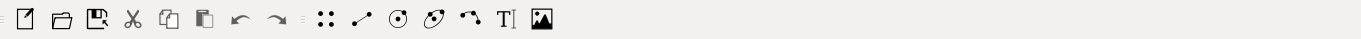
\includegraphics[width=0.9\textwidth]{images/toolbar.png}
\caption{Toolbar}
\end{figure}
Toolbar contains the shortcut of the various items in menubar. Like new, open, save, close, undo, redo etc. There are two toolbar standard toolbar and main toolbar.
\begin{enumerate}
\item \textbf{Main Toolbar}
\begin{figure}[h!]

\includegraphics[width=0.05\textwidth]{images/newDrawing.jpg} 
This creates a new Document.
\end{figure}
\begin{figure}[h!]

\includegraphics[width=0.05\textwidth]{images/openDrawing.jpg} 
This opens a document.
\end{figure}
\begin{figure}[h!]

\includegraphics[width=0.05\textwidth]{images/saveDrawing.jpg} 
This saves a document.
\end{figure}
\begin{figure}[h!]

\includegraphics[width=0.05\textwidth]{images/cut.jpg} 
This cuts the selected entity.
\end{figure}
\begin{figure}[h!]

\includegraphics[width=0.05\textwidth]{images/copy.jpg} 
This copies the selected entity.
\end{figure}
\begin{figure}[h!]

\includegraphics[width=0.05\textwidth]{images/paste.jpg} 
This paste the entity at the position.
\end{figure}
\begin{figure}[h!]

\includegraphics[width=0.05\textwidth]{images/undo.jpg} 
This undo the previous action.
\end{figure}
\begin{figure}[h!]

\includegraphics[width=0.05\textwidth]{images/redo.jpg} 
This redo the previous action.
\end{figure}
\item \textbf{Standard ToolBar}
\begin{figure}[h!]

\includegraphics[width=0.05\textwidth]{images/point.jpg} 
This will create points
\end{figure}
\begin{figure}[h!]

\includegraphics[width=0.05\textwidth]{images/line.jpg} 
This will create line
\end{figure}
\begin{figure}[h!]

\includegraphics[width=0.05\textwidth]{images/circle.jpg} 
This will create circle
\end{figure}
\begin{figure}[h!]

\includegraphics[width=0.05\textwidth]{images/ellipse.jpg} 
This will create ellipse
\end{figure}
\begin{figure}[h!]

\includegraphics[width=0.05\textwidth]{images/arc.jpg} 
This will create arc
\end{figure}
\begin{figure}[h!]

\includegraphics[width=0.05\textwidth]{images/text.jpg} 
This will create a box to insert text
\end{figure}
\begin{figure}[h!]

\includegraphics[width=0.05\textwidth]{images/image.jpg} 
This will insert image
\end{figure}
\end{enumerate}
\vspace{30em}
\subsection{Working Space}
\begin{figure}[h!]
\centering
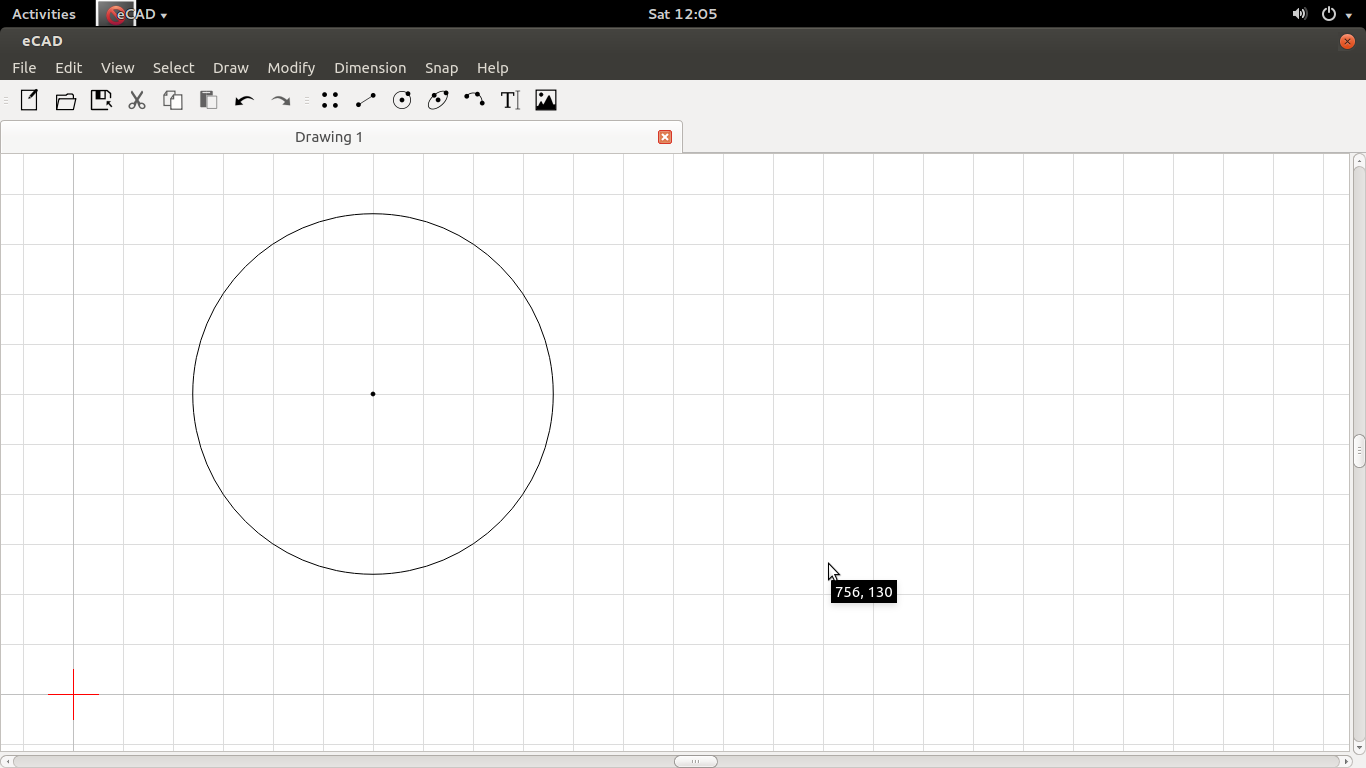
\includegraphics[width=0.9\textwidth]{images/drawingarea.png} 
\caption{Working Space}
\end{figure}
This is the working space where all the entities are drawn. We can increase or decrese the working area by closing or opening the widgets like scripting console and status bar. At present the are closed. This is the maximum area one will get to work. One can also make more than one document so that he/she can work easily. All depends upon user need.
\subsection{Scipting Console}
\begin{figure}[h!]
\centering
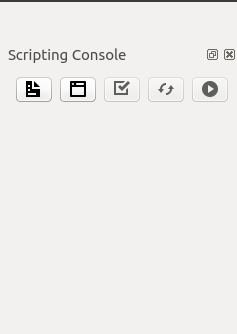
\includegraphics[width=0.4\textwidth]{images/scriptingconsole.png} 
\caption{Scripting console}
\end{figure}
In scripting console user can write the script/code to draw the drawing. So this feature is effective for technical user, who is excited and want to code. The code for each entity is very simple. There are different icons of in scripting. Each have its different meaning.
\begin{figure}[h!]

\includegraphics[width=0.05\textwidth]{images/document.png} 
This will create a new document in scripting console.
\end{figure}
\begin{figure}[h!]

\includegraphics[width=0.05\textwidth]{images/browser.png} 
This will load an existing script
\end{figure}
\begin{figure}[h!]

\includegraphics[width=0.05\textwidth]{images/task.png} 
This will save the script which is written.
\end{figure}
\begin{figure}[h!]

\includegraphics[width=0.05\textwidth]{images/loop-circular.png} 
This will clear the existing script.
\end{figure}
\begin{figure}[h!]

\includegraphics[width=0.05\textwidth]{images/play-circular.png} 
This will execute the current script.
\end{figure}
\newpage
\subsection{Status Bar}
\begin{figure}[h!]
\centering
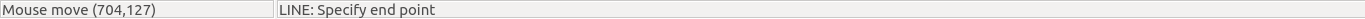
\includegraphics[width=0.9\textwidth]{images/statusbar.png} 
\caption{Status Bar}
\end{figure}
The status bar tells us aout two things
\begin{itemize}
\item Current screen position
\item What to do next while making an entity through UI part.
\end{itemize}